\documentclass[10pt,preprint]{aastex}

\usepackage{amsfonts}
\usepackage{amsmath}
\usepackage{amssymb}
\usepackage{amsthm}
\usepackage{booktabs}
\usepackage{mathrsfs}
\usepackage{cite}
\usepackage{times}
\usepackage{url}
\usepackage{hyperref}
\usepackage{lineno}
\usepackage{yhmath}
\usepackage{natbib}
\usepackage{../definitions}
\hypersetup{
  bookmarksnumbered = true,
  bookmarksopen=false,
  pdfborder=0 0 0,         % make all links invisible, so the pdf looks good when printed
  pdffitwindow=true,      % window fit to page when opened
  pdfnewwindow=true, % links in new window
  colorlinks=true,           % false: boxed links; true: colored links
  linkcolor=blue,            % color of internal links
  citecolor=magenta,    % color of links to bibliography
  filecolor=magenta,     % color of file links
  urlcolor=cyan              % color of external links
}

\usepackage{graphicx}
\graphicspath{ {Figures/} }

\newcommand{\ee}[1]{{\color{red} #1}}
\newcommand{\dx}{\Delta x}
\newcommand{\pbK}{\partial\mathbf{K}}
\newcommand{\sumx}{\sum_{i=1}^{d}}

\begin{document}

\title{Nodal Discontinuous Galerkin Method for the Euler Equations of Fluid Dynamics}
\author{Eirik Endeve\altaffilmark{1}, et al.}
\altaffiltext{1}{Computational and Applied Mathematics Group, Oak Ridge National Laboratory, Oak Ridge, TN 37831-6354, USA; endevee@ornl.gov}

\begin{abstract}
We present a nodal Discontinuous Galerkin (DG) method for the Euler equations with an eye towards astrophysical hydrodynamics.  
We focus on issues related to core-collapse supernova dynamics, which include the use of curvilinear coordinates and a non-ideal (nuclear) equation of state.  
\end{abstract}

\tableofcontents

\section{Introduction}

\clearpage

\section{Euler Equations of Gas Dynamics in Curvilinear Coordinates}

\subsection{Basic Mathematical Model}

For general curvilinear spatial coordinates, the non-relativistic Euler equations for gas dynamics are %\citep[][see, e.g., \citet{} and references therein for a fully general relativistic treatment]{leveque_2002}
\begin{equation}
  \pderiv{\rho}{t}
  +\f{1}{\sqrt{\gamma}}\pderiv{}{x^{i}}\Big(\,\sqrt{\gamma}\,\rho\,v^{i}\,\Big)=0,
  \label{eq:massConservation}
\end{equation}
\begin{equation}
  \pderiv{S_{j}}{t}
  +\f{1}{\sqrt{\gamma}}\pderiv{}{x^{i}}\Big(\,\sqrt{\gamma}\,P^{i}_{~j}\,\Big)
  =\f{1}{2}\,P^{ik}\,\pderiv{\gamma_{ik}}{x^{j}}-\rho\,\pderiv{\Phi}{x^{j}},
  \label{eq:momentumConservation}
\end{equation}
\begin{equation}
  \pderiv{E}{t}
  +\f{1}{\sqrt{\gamma}}\pderiv{}{x^{i}}\Big(\,\sqrt{\gamma}\,\big(E+p\big)\,v^{i}\,\Big)
  =-S^{i}\,\pderiv{\Phi}{x^{i}},
  \label{eq:energyConservation}
\end{equation}
\begin{equation}
  \pderiv{n_{e}}{t}
  +\f{1}{\sqrt{\gamma}}\pderiv{}{x^{i}}\Big(\,\sqrt{\gamma}\,n_{e}\,v^{i}\,\Big)=0,
  \label{eq:electronConservation}
\end{equation}
where $\rho$ is the (baryon) mass density, $S^{i}=\rho\,v^{i}$ is the momentum density, $P^{ij}=\rho\,v^{i}\,v^{j}+p\,\gamma^{ij}$ the stress tensor, $E=e+\f{1}{2}\,\rho\,v_{i}\,v^{i}$ the total (internal plus kinetic) energy density, and $n_{e}$ the electron density.  
The pressure is related to the density, internal energy density, and electron density by an equation of state (EoS); i.e., $p=p(\rho,e,n_{e})$.  
(We also define the specific internal energy by $\epsilon=e/\rho$.)
The Newtonian gravitation potential, $\Phi$, is obtained from solving
\begin{equation}
  \f{1}{\sqrt{\gamma}}\pderiv{}{x^{i}}\Big(\,\sqrt{\gamma}\,\gamma^{ij}\pderiv{\Phi}{x^{j}}\,\Big)=4\pi\,\rho.  
  \label{eq:poisson}
\end{equation}

The model given by Eqs.~\eqref{eq:massConservation} - \eqref{eq:electronConservation} is non-relativistic (i.e., it does not include effects due to strong gravitational fields or relativistic fluid velocities), but is expressed in terms of curvilinear coordinates through the spatial metric tensor $\gamma_{ij}$, which gives squared infinitesimal line-element
\begin{equation}
  ds_{\vect{x}}^{2}=\gamma_{ij}\,dx^{i}\,dx^{j},
\end{equation}
where $\gamma_{ij}$ are the spatial components of the coordinate basis metric tensor.  
We will make two simplifying assumptions: the metric tensor is (1) diagonal and (2) time-independent.  
Specifically we assume the following diagonal form
\begin{equation}
  \gamma_{ij}
  =\mbox{diag}\big[\,\gamma_{11},\,\gamma_{22}(x^{1}),\,\gamma_{33}(x^{1},x^{2})\,\big], 
  \label{eq:threeMetric}
\end{equation}
which is sufficiently general to accommodate Cartesian, cylindrical, and spherical polar coordinates (see Table~\ref{tab:metricFunctions} and Appendix~\ref{app:CurvilinearEuler}).  
Moreover, $\gamma$ is the determinant of the metric tensor; $\sqrt{\gamma}=\sqrt{\gamma_{11}\gamma_{22}\gamma_{33}}$.  
The inverse of the spatial metric is denoted $\gamma^{ij}$, so that $\gamma^{ik}\gamma_{kj}=\delta^{i}_{~j}$.  
We can use the spatial metric to raise and lower indices on spatial vectors and tensors; e.g., $S_{j}=\gamma_{jk}\,S^{k}$.  

\begin{table}
  \begin{center}
  \caption{Relevant metric functions for Cartesian, Cylindrical, and Spherical coordinate systems.\label{tab:metricFunctions}}
  \begin{tabular}{ccccccccccc}
    \midrule
    Coordinates & $x^{1}$ & $x^{2}$ & $x^{3}$ & $\gamma_{11}$ & $\gamma_{22}$ & $\gamma_{33}$ & $\sqrt{\gamma}$
    & $\f{1}{\gamma_{22}}\pderiv{\gamma_{22}}{x^{1}}$ & $\f{1}{\gamma_{33}}\pderiv{\gamma_{33}}{x^{1}}$ & $\f{1}{\gamma_{33}}\pderiv{\gamma_{33}}{x^{2}}$ \\
    \midrule
    \midrule
    Cartesian  & $x$ & $y$ & $z$ & 1 & 1 & 1 & 1 & 0 & 0 & 0 \\
    Cylindrical & $R$ & $z$ & $\phi$ & 1 & 1 & $R^{2}$ & $R$ & 0 & $2/R$ & 0 \\
    Spherical   & $r$ & $\theta$ & $\phi$ & 1 & $r^{2}$ & $r^{2}\sin^{2}\theta$ & $r^{2}\sin\theta$ & $2/r$ & $2/r$ & $2\cot\theta$ \\
    \midrule
    \midrule
  \end{tabular}
  \end{center}
\end{table}

\subsection{Euler Equations as a System of Conservation Laws with Sources}

We define the geometry sources in Eq.~\eqref{eq:momentumConservation} by
\begin{equation}
  G_{j}
  =\f{1}{2}\,P^{ik}\,\pderiv{\gamma_{ik}}{x^{j}}-\rho\,\pderiv{\Phi}{x^{j}}.  
\end{equation}
Specifically, using the time-independent metric tensor in Eq.~\eqref{eq:threeMetric} and writing in terms of $P^{i}_{~j}$, the components are
\begin{equation}
  G_{1}
  =\f{1}{2}\,\Big(\,P^{2}_{~2}\,\f{1}{\gamma_{22}}\pderiv{\gamma_{22}}{x^{1}}+P^{3}_{~3}\,\f{1}{\gamma_{33}}\pderiv{\gamma_{33}}{x^{1}}\,\Big)-\rho\,\pderiv{\Phi}{x^{1}}, \quad
  G_{2}
  =\f{1}{2}\,P^{3}_{~3}\,\f{1}{\gamma_{33}}\pderiv{\gamma_{33}}{x^{2}}-\rho\,\pderiv{\Phi}{x^{2}}, \quad\text{and}\quad
  G_{3}
  =-\rho\,\pderiv{\Phi}{x^{3}}.
\end{equation}
The gravitational energy source term in Eq.~\eqref{eq:energyConservation} is denoted with $G_{E}=-S^{i}\,\pd{\Phi}{x^{i}}$.  

Then, by defining the vector of evolved variables $\bU=\big(\,\rho,\,S_{1},\,S_{2},\,S_{3},\,E,\,n_{e}\,\big)^{T}$, the vector of geometry sources $\bG(\bU)=\big(\,0,\,G_{1},\,G_{2},\,G_{3},\,G_{E},\,0\,\big)^{T}$, and the flux vector components
\begin{equation}
  \vect{F}^{i}(\bU)
  =\big(\,\rho\,v^{i},\,P_{~1}^{i},\,P_{~2}^{i},\,P_{~3}^{i},\,(E+p)\,v^{i},\,n_{e}\,v^{i}\,\big)^{T},
\end{equation}
we write the system of equations in the usual compact form
\begin{equation}
  \pd{\bU}{t}
  +\f{1}{\sqrt{\gamma}}\pderiv{}{x^{i}}\Big(\,\sqrt{\gamma}\,\vect{F}^{i}(\bU)\,\Big)
  =\bG(\bU).
  \label{eq:extendedEulerCompact}
\end{equation}
Eq.~\eqref{eq:extendedEulerCompact} forms the basis for developing DG methods for the Euler equations.  

\section{Discontinuous Galerkin Discretization}

In the DG method, the conserved quantities are approximated by a local expansion of the form
\begin{equation}
  \bU_{\DG}(\bx,t)
  =\sum_{\bi=\vect{1}}^{\bN}\bU_{\bi}(t)\,\ell_{\bi}(\bx), 
\end{equation}
where basis functions $\ell_{\bi}(\bx)$, which we will take to be polynomials, belong to a function space denoted $\bbV^{k}$ and have local support in a computational cell or element denoted by $\bK$.  

Several books and review articles on the DG method are now available \citep[see, e.g.,][]{cockburnShu_2001,hesthavenWarburton_2008}, and we will not go into too much detail here.  
However, we review some key concepts to introduce notation, and emphasize specific choices in our implementation.  

\subsection{Basic Principles of the DG Method}

We divide the computational domain $D$ into a disjoint union $\mathcal{T}$ of open elements $\bK$, so that $D = \cup_{\bK \in \cT}\bK$.  
We require that each element is a box in the logical coordinates; i.e.,
\begin{equation}
  \bK=\{\vect{x} : x^{i} \in K^{i} := (\xL^{i},\xH^{i})\}, 
\end{equation}
with the surface elements denoted $\pbK^{i}=\otimes_{j\ne i}K^{j}$.  
We use $V_{\bK}$ to denote the proper volume of the element
\begin{equation}
  V_{\bK} = \int_{\bK}dV, \quad\text{where}\quad dV = \sqrt{\gamma}\,\prod_{i=1}^{d}dx^{i}.  
\end{equation}
We also define $\bx=\{\tilde{\bx}^{i},x^{i}\}$ and $\dx^{i}=\xH^{i}-\xL^{i}$.  

We let the approximation space for the DG method, $\mathbb{V}^{k}$, to be constructed from the tensor product of one-dimensional polynomials of maximal degree $k$.  
Note that functions in $\mathbb{V}^{k}$ can be discontinuous across element interfaces.  
The semi-discrete DG problem is to find $\bU_{\DG}\in\mathbb{V}^{k}$ (which approximates $\bU$) such that
\begin{align}
  &\partial_{t}\int_{\bK}\bU_{\DG}\,v\,dV
  +\sumx\int_{\pbK^{i}}\big(\,\sqrt{\gamma}\,\widehat{\vect{F}}^{i}(\bU_{\DG})\,v\big|_{\xH^{i}}-\sqrt{\gamma}\,\widehat{\vect{F}}^{i}(\bU_{\DG})\,v\big|_{\xL^{i}}\,\big)\,d\tilde{\bx}^{i} \nonumber \\
  &\hspace{24pt}
  -\sumx\int_{\bK}\vect{F}^{i}(\bU_{\DG})\,\pderiv{v}{x^{i}}\,dV
  =\int_{\bK}\bG(\bU_{\DG})\,v\,dV
  \label{eq:semidiscreteDG}
\end{align}
for all $v\in\mathbb{V}^{k}$ and all $\bK\in\mathcal{T}$.  

To connect the elements in Eq.~\eqref{eq:semidiscreteDG}, $\widehat{\bF}^{i}(\bU_{\DG})$ is a numerical flux approximating the flux on the $i$th surface of $\bK$.  
For this purpose we define the numerical flux function $\vect{f}^{i}$, which evaluates the numerical flux given values from both sides of an element interface; i.e.,
\begin{equation}
  \widehat{\bF}^{i}(\bU_{\DG})=\vect{f}^{i}(\bU_{\DG}(x^{i,-},\tilde{\bx}^{i}),\bU_{\DG}(x^{i,+},\tilde{\bx}^{i})),
\end{equation}
where superscripts $-/+$, e.g., in the arguments of $\bU_{\DG}(x^{i,-/+},\tilde{\bx}^{i})$, indicate that the function is evaluated to the immediate left/right of $x^{i}$.  
For example, the simple Lax-Friedrichs flux is given by
\begin{equation}
  \vect{f}^{i}(\bU^{-},\bU^{+})
  =\f{1}{2}\,\big(\,\bF^{i}(\bU^{-})+\bF^{i}(\bU^{+})-\alpha^{i}\,(\,\bU^{+}-\bU^{-}\,)\,\big),
\end{equation}
where $\alpha^{i}=||\mbox{eig}\big(\partial\bF^{i}/\partial\bU\big)||_{\infty}$ is the largest eigenvalue of the flux jacobian.  
We have implemented the Local Lax-Friedrichs flux, the Harten-Lax-van Leer (HLL) flux, and the HLLC flux, but use the HLLC flux for all the numerical experiments presented in Sections~\ref{sec:NumericalExperiments} and \ref{sec:MiniApp}.  

The approximation space $\mathbb{V}^{k}$ contains the constant functions, and the choice $v=1$ in Eq.~\eqref{eq:semidiscreteDG} gives
\begin{equation}
  \partial_{t}\bU_{\bK}
  +\f{1}{V_{\bK}}\sumx\int_{\pbK^{i}}\big(\,\sqrt{\gamma}\,\widehat{\vect{F}}^{i}(\bU_{\DG})\big|_{\xH^{i}}-\sqrt{\gamma}\,\widehat{\vect{F}}^{i}(\bU_{\DG})\big|_{\xL^{i}}\,\big)\,d\tilde{\bx}^{i}
  =\bG_{\bK},
\end{equation}
where we have defined the volume averages
\begin{equation}
  \bU_{\bK}=\f{1}{V_{\bK}}\int_{\bK}\bU_{\DG}\,dV \quad\text{and}\quad
  \bG_{\bK}=\f{1}{V_{\bK}}\int_{\bK}\bG(\bU_{\DG})\,dV.  
\end{equation}
This illustrates how the cell average (similar to finite volume methods) is evolved in the DG method.  

\subsection{Further Details on the DG Discretization of the Euler Equations}

Here we provide further details on the DG method in order to arrive at the equations that are actually implemented in our code.  
We start by introducing some notation, defining the polynomial expansion for $\bcM_{\DG}$, and the quadrature rules used to evaluate the integrals in Equation~\eqref{eq:semidiscreteDG}.  
Then, using these rules, we provide explicit expressions for each of the terms in Equation~\eqref{eq:semidiscreteDG}.  

\subsubsection{Notation and Definitions}

In each element $\bK$, we use a nodal representation in the conserved variables $\bU$; i.e.,
\begin{equation}
  \bU(\bx,t)\approx
  \bU_{\DG}(\bx,t)=\sum_{\bi=\vect{1}}^{\bN}\bU_{\bi}(t)\,\ell_{\bi}(\bx),
  \label{eq:conservedNodalExpansion}
\end{equation}
where $\ell_{\bi}(\bx)\in\bbQ^{k}$ are basis functions.  
Specifically, we use one-dimensional Lagrange polynomials $\ell_{i}(x)$ to construct the multidimensional representation, where
\begin{equation}
  \ell_{i}(\eta)=
  \prod_{\substack{j=1\\j\ne i}}^{N}\f{\eta-\eta_{j}}{\eta_{i}-\eta_{j}}.  
\end{equation}
Moreover $\bi=\{i_{1},\ldots,i_{d}\}$ is a multi-index, and $\ell_{\bi}(\bx)=\prod_{k=1}^{d}\ell_{i_{k}}(x^{k})$.  
From the property $\ell_{i}(x_{j})=\delta_{ij}$ we have the corresponding multidimensional version $\ell_{\bi}(\bx_{\bj})=\delta_{\bi\bj}$, so that $\bU_{\DG}(\bx_{\bi},t)=\bU_{\bi}(t)$; i.e., the expansion coefficients in Equation \eqref{eq:conservedNodalExpansion} represent the conserved variables defined in the nodes $\bx_{\bi}$.  
To evaluate the integrals in Equation~\eqref{eq:semidiscreteDG}, we introduce numerical quadratures.  
First we define the one-dimensional $N$-point quadrature $Q_{N}^{i}:C^{0}(I^{i})\to\bbR$ with abscissas $\{\eta_{q}\}_{q=1}^{N}$ and weights $\{w_{q}\}_{q=1}^{N}$, normalized such that $\sum_{q=1}^{N}w_{q}=1$.  
(For example, the $N$-point Legendre-Gauss quadrature, which we will use, integrates polynomials of degree $\le 2N-1$ exactly.)
If $P(x)$ is such a polynomial, we have
\begin{equation}
  \f{1}{\Delta x}\int_{K}P(x)\,dx=\int_{I}P(\eta)\,d\eta=Q_{N}\big[P\big]\equiv\sum_{q=1}^{N}w_{q}\,P(\eta_{q}).  
\end{equation}

Multi-dimensional integrals are evaluated by tensorization of one-dimensional quadratures.  
For volume integrals, we define $\bQ_{N}:C^{0}(\bI)\to\bbR$ as the tensor product of one-dimensional $N$-point Legendre-Gauss quadrature rules $\bQ_{N}=\otimes_{i=1}^{d}Q_{N}^{i}$ with abscissas $\{\vect{\eta}_{\bq}\}_{\bq=\vect{1}}^{\bN}$ and weights $\{w_{\bq}\}_{\bq=\vect{1}}^{\bN}$.  
Here, $\bq=\{q_{i}\}_{i=1}^{d}\in\bbN^{d}$, $\vect{\eta}_{\bq}=\{\eta_{q_{1}}^{1},\ldots,\eta_{q_{d}}^{d}\}$, and $w_{\bq}=w_{q_{1}}\ldots w_{q_{d}}$, so that the multi-dimensional volume integral is evaluated as
\begin{equation}
  \f{1}{|\bK|}\int_{\bK}P(\bx)\,d\bx
  =\int_{\bI}P(\vect{\eta})\,d\vect{\eta}
  =\bQ_{N}\big[P\big]
  \equiv\sum_{\bq=\vect{1}}^{\bN}w_{\bq}\,P(\vect{\eta}_{\bq}),
\end{equation}
where $P:\bbR^{d}\to\bbR$.  
Similarly, for surface integrals, we define $\tilde{\bQ}_{N}^{i}:C^{0}(\tilde{\bI}^{i})\to\bbR$ as the tensor product $\tilde{\bQ}_{N}^{i}=\otimes_{j\ne i}Q_{N}^{j}$ and denote the abscissas with $\{\tilde{\vect{\eta}}_{\tilde{\bq}_{i}}^{i}\}_{\tilde{\bq}_{i}=\vect{1}}^{\bN}$ and the weights with $\{w_{\tilde{\bq}_{i}}\}_{\tilde{\bq}_{i}=\vect{1}}^{\bN}$, respectively.  
Here, the multi-index is $\tilde{\bq}_{i}=\{q_{j}\}_{j\ne i}\in\bbN^{d-1}$, $\tilde{\vect{\eta}}_{\tilde{\bq}_{i}}^{i}=\{\eta_{q_{j}}^{j}\}_{j\ne i}$, and $w_{\tilde{\bq}_{i}}=\prod_{j\ne i}w_{q_{j}}$.  
Surface integrals are then evaluated as
\begin{equation}
  \f{1}{|\tilde{\bK}^{i}|}\int_{\tilde{\bK}^{i}}P(x^{i},\tilde{\bx}^{i})\,d\tilde{\bx}^{i}
  =\int_{\tilde{\bI}^{i}}P(x^{i},\tilde{\vect{\eta}}^{i})\,d\tilde{\vect{\eta}}^{i}
  =\tilde{\bQ}_{N}^{i}\big[P\big]
  \equiv\sum_{\tilde{\bq}_{i}=\vect{1}}^{\bN}w_{\tilde{\bq}_{i}}\,P(x^{i},\tilde{\vect{\eta}}_{\tilde{\bq_{i}}}^{i}).  
\end{equation}

\subsubsection{Explicit Expressions}

Inserting \eqref{eq:conservedNodalExpansion} into \eqref{eq:semidiscreteDG}, with $v(\bx)=\ell_{\bk}(\bx)$ and the quadratures defined above, we obtain
\begin{align}
  \pd{}{t}\int_{\bK}\bU_{\DG}\,v\,dV
  &\approx w_{\bk}\,\sqrt{\gamma}_{\bk}\,\pd{}{t}\bU_{\bk}\,|\bK|
\end{align}
for the time derivative term, where $|\bK|=\prod_{i=1}^{d}\Delta x^{i}$.  
The integration is approximate since we use the Legendre-Gauss quadrature rule with the nodal points given by the expansion in Eq.~\eqref{eq:conservedNodalExpansion}.  
This leads to a diagonal mass matrix, and simplifies the implementation.  
Similarly, we obtain
\begin{align}
  \int_{\bK}\bG(\bU_{\DG})\,v\,dV
  &\approx w_{\bk}\,\sqrt{\gamma}_{\bk}\,\bG(\bU_{\bk})\,|\bK|.
\end{align}
for the source term.  
The gravitational source terms warrants some additional exposition, which we defer to Section~\ref{sec:sourceTerms}.  

For the surface integrals, we obtain, e.g., 
\begin{equation}
  \int_{\pbK^{i}}\sqrt{\gamma}\,\widehat{\vect{F}}^{i}\,v\big|_{\xH^{i}}\,d\tilde{\bx}^{i}
  \approx w_{\tilde{\bk}_{i}}\,\sqrt{\gamma}(x_{\Hgh}^{i},\tilde{\bx}_{\tilde{\bk}_{i}}^{i})\,\widehat{\bF}^{i}(x_{\Hgh}^{i},\tilde{\bx}_{\tilde{\bk}_{i}}^{i})\,\ell_{k_{i}}(\eta_{\Hgh}^{i})\,|\tilde{\bK}^{i}|,
\end{equation}
where $|\tilde{\bK}^{i}|=\prod_{j\ne i}\Delta x^{j}$.  
(Note: we do not use Einstein's summation convention in the numerical expressions presented in this section.  
Summation over indices will be explicitly indicated.)  
Finally, the volume term becomes
\begin{equation}
  \int_{\bK}\bF^{i}\,\pderiv{v}{x^{i}}\,dV
  \approx w_{\tilde{\bk}_{i}}\sum_{q_{i}=1}^{N}
  w_{q_{i}}\,\sqrt{\gamma}(x_{q_{i}}^{i},\tilde{\bx}_{\tilde{\bk}_{i}}^{i})\,\bF^{i}(x_{q_{i}}^{i},\tilde{\bx}_{\tilde{\bk}_{i}}^{i})\,\pderiv{\ell_{k_{i}}}{\eta^{i}}(\eta_{q_{i}}^{i})\,|\tilde{\bK}^{i}|.
\end{equation}
Combining the terms and dividing though by $w_{\bk}\,\sqrt{\gamma}_{\bk}\,|\bK|$, we obtain the semi-discrete for of the Euler equations
\begin{align}
  \pd{}{t}\bU_{\bk}
  &=
  -\f{1}{\sqrt{\gamma}_{\bk}}
  \sum_{i=1}^{d}\f{1}{w_{k_{i}}\,\Delta x^{i}}\,
  \Big(\,
    \sqrt{\gamma}(x_{\Hgh}^{i},\tilde{\bx}_{\tilde{\bk}_{i}}^{i})\,\widehat{\bF}^{i}(x_{\Hgh}^{i},\tilde{\bx}_{\tilde{\bk}_{i}}^{i})\,\ell_{k_{i}}(\eta_{\Hgh}^{i})
    -\sqrt{\gamma}(x_{\Low}^{i},\tilde{\bx}_{\tilde{\bk}_{i}}^{i})\,\widehat{\bF}^{i}(x_{\Low}^{i},\tilde{\bx}_{\tilde{\bk}_{i}}^{i})\,\ell_{k_{i}}(\eta_{\Low}^{i})
  \,\Big) \nonumber \\
  &\hspace{12pt}
  +\f{1}{\sqrt{\gamma}_{\bk}}
  \sum_{i=1}^{d}\f{1}{w_{k_{i}}\,\Delta x^{i}}\sum_{q_{i}=1}^{N}w_{q_{i}}\,\sqrt{\gamma}(x_{q_{i}}^{i},\tilde{\bx}_{\tilde{\bk}_{i}}^{i})\,\bF^{i}(x_{q_{i}}^{i},\tilde{\bx}_{\tilde{\bk}_{i}}^{i})\,\pderiv{\ell_{k_{i}}}{\eta^{i}}(\eta_{q_{i}}^{i})
  +\bG(\bU_{\bk})
  \label{eq:semidiscreteDiscretized}
\end{align}
Equation~\eqref{eq:semidiscreteDiscretized} provides the basis for implementation in our code.  

\subsubsection{Reconstruction to Element interfaces}

\begin{equation}
  \bU_{\DG}(\eta_{\Low}^{i},\tilde{\vect{\eta}}_{\tilde{\bq}_{i}}^{i})
  =\sum_{\bk=\vect{1}}^{\bN}\bU_{\bk}\,\ell_{\bk}(\eta_{\Low}^{i},\tilde{\vect{\eta}}_{\tilde{\bq}_{i}}^{i})
  =\sum_{k_{i}=1}^{N}\sum_{\tilde{\bk}_{i}=\vect{1}}^{\bN}\bU_{(k_{i},\tilde{\bk}_{i})}\,\ell_{k_{i}}(\eta_{\Low}^{i})\,\ell_{\tilde{\bk}_{i}}(\tilde{\vect{\eta}}_{\tilde{\bq}_{i}}^{i})
\end{equation}

\subsubsection{The One-Dimensional Case}

Here we simplify the DG discretization in Eq.~\eqref{eq:semidiscreteDiscretized} to the one-dimensional ($d=1$) case to make the notation more transparent.  
With $d=1$, we substitute $\bk\to k_{d}\to k$, $x^{d}\to x$, $q_{i}\to q$, etc., so that Eq.~\eqref{eq:semidiscreteDiscretized} reduces to
\begin{align}
  \pd{}{t}\bU_{k}
  &=-\f{1}{\sqrt{\gamma}_{k}}
  \f{1}{w_{k}\,\Delta x}\,
  \Big(\,
    \sqrt{\gamma}(x_{\Hgh})\,\widehat{\bF}(x_{\Hgh})\,\ell_{k}(\eta_{\Hgh})
    -\sqrt{\gamma}(x_{\Low})\,\widehat{\bF}(x_{\Low})\,\ell_{k}(\eta_{\Low})
  \,\Big) \nonumber \\
  & \hspace{12pt}
  +\f{1}{\sqrt{\gamma}_{k}}
  \f{1}{w_{k}\,\Delta x}\sum_{q=1}^{N}w_{q}\,\sqrt{\gamma}(x_{q})\,\bF(x_{q})\,\pderiv{\ell_{k}}{\eta}(\eta_{q})
  +\bG(\bU_{k}).
  \label{eq:semidiscreteDiscretized1D}
\end{align}

\subsection{Source Terms}
\label{sec:sourceTerms}

\section{Time Integration}
\label{sec:TimeIntegration}

For time integration, we employ the strong stability-preserving Runge-Kutta (SSP-RK) methods \citep[e.g.,][]{gottlieb_etal_2001}, which, for evolving the Euler equations from $t^{n}$ to $t^{n+1}=t^{n}+\dt$ ($\bU^{n}\to\bU^{n+1}$) using $m$ stages, take the general form
\begin{align}
  \bU^{(0)}
  &=\bU^{n}, \\
  \bU^{(i)}
  &=\sum_{k=0}^{i-1}\alpha_{ik}\,\big[\,\bU^{(k)}+\beta_{ik}\,\dt\,\bcL(\bU^{(k)})\,\big], \quad i=1,\ldots,m 
  \label{eq:ssprkStages} \\
  \bU^{n+1}
  &=\bU^{(m)}.  
\end{align}
For second- and third-order temporal accuracy (denoted SSP-RK2 and SSP-RK3, respectively), the coefficient matrices $\alpha_{ik}$ and $\beta_{ik}$ are given by \citep{shuOsher_1988}.  
Note that $\alpha_{ik},\beta_{ik}\ge0$ and $\sum_{k}\alpha_{ik}=1~\forall i$, so that the RK stages in Eq.~\eqref{eq:ssprkStages} are simply convex combinations of forward Euler steps with time step $\beta_{ik}\,\dt$.  

\section{Equation of State (EoS)}

\section{Polynomial Limiting}

\subsection{Slope Limiters}

\subsection{Positivity Limiters}

In the case of the nuclear EoS, the thermodynamic quantities (e.g, pressure) are tabulated in terms of mass density $\rho$, temperature $T$, and electron fraction $Y_{e}$.  
Obviously, the tables are of finite extent in these independent variables; i.e., $\rho\in[\rho_{0},\rho_{1}]$, $T\in[T_{0},T_{1}]$, and $Y_{e}\in[Y_{e,0},Y_{e,1}]$.  
During stellar core-collapse, the internal energy density has a dominant contribution from degenerate electrons, which is independent of the temperature.  
During core bounce and shock formation, we have found that the numerical scheme (e.g., during reconstruction of element interfaces) can lead to internal energy densities that fall below the lower boundary of the tabulated data and failure to obtain a temperature, which is needed to evaluate the pressure.  
(Extending the table to lower values of temperature does not help since the internal energy density is practically independent of the temperature.)

For the solution to the Euler equations, we define the set of physically admissible states as
\begin{equation}
  \cG=\big\{\,\bU~|~\rho\ge\rho_{0}, e\ge e_{0}(\rho,T_{0},n_{e}),n_{e}\ge n_{e,0}(\rho,Y_{e,0})\,\big\}
\end{equation}


\section{Gravity Solver: Finite Element Method}
\label{sec:FiniteElementMethod}

To solve Poisson's equation given by Eq.~\eqref{eq:poisson}, we use the finite element method (FEM).  
\ee{Nick fills in here}.  

\section{Benchmark Problems}
\label{sec:NumericalExperiments}

We benchmark the DG implementation against a series of test problems.  
We will vary the degree $k$ of the polynomial representation from 0 to 3, which we then denote DG($k$).  
IWe use the explicit SSP-RK time integrators in Section~\ref{sec:explicitTime}.  
The 2-stage and 3-stage methods are denoted SSP-RK2 and SSP-RK3, respectively.  
As an example, an expected third-order accurate method (for problems with smooth solutions), using DG(2) and SSP-RK3, will then be denoted DG(2)+RK3.  
We use the finite element method in Section~\ref{sec:FiniteElementMethod} with the same polynomial degree as the DG method for problems involving self-gravity.  

\subsection{Smooth Problem: Linear Waves}

\subsubsection{Entropy Waves (Accuracy Test)}

\begin{table}
  \begin{center}
  \caption{$L^{\infty}$ error and convergence rates for the entropy wave problem.}
  \label{tab:streamingSineWave}
  \begin{tabular}{ccccccccc}
    & \multicolumn{4}{c}{SSP-RK2} & \multicolumn{4}{c}{SSP-RK3} \\
    \cmidrule(r){2-5} \cmidrule(r){6-9}
    $N$ & DG(1) & Rate & DG(2) & Rate & DG(2) & Rate & DG(3) & Rate \\
    \midrule \midrule
    8     & $1.766\times10^{-1}$ & ---  & $2.371\times10^{-3}$ & ---  & $1.700\times10^{-3}$ & ---  & $4.958\times10^{-5}$  & --- \\
    16   & $2.893\times10^{-2}$ &2.61& $3.236\times10^{-4}$ &2.87& $1.300\times10^{-4}$ &3.71& $3.044\times10^{-6}$ &4.03 \\
    32   & $4.203\times10^{-3}$ &2.78& $6.800\times10^{-5}$ &2.25& $1.580\times10^{-5}$ &3.04& $1.983\times10^{-7}$ &3.94 \\
    64   & $6.455\times10^{-4}$ &2.70& $1.542\times10^{-5}$ &2.14& $1.971\times10^{-6}$ &3.00& $1.343\times10^{-8}$ &3.88 \\
    128 & $1.101\times10^{-4}$ &2.55& $3.659\times10^{-6}$ &2.08& $2.464\times10^{-7}$ &3.00& $9.737\times10^{-10}$ &3.79 \\
    256 & $2.109\times10^{-5}$ &2.38& $8.904\times10^{-7}$ &2.04& $3.081\times10^{-8}$ &3.00& $9.012\times10^{-11}$ &3.43 \\
    \midrule \midrule
  \end{tabular}
  \end{center}
\end{table}

\subsubsection{Sound Waves}

\subsection{Riemann Problems}

\subsubsection{Shock Tube}

\begin{figure}[h]
  \begin{center}
     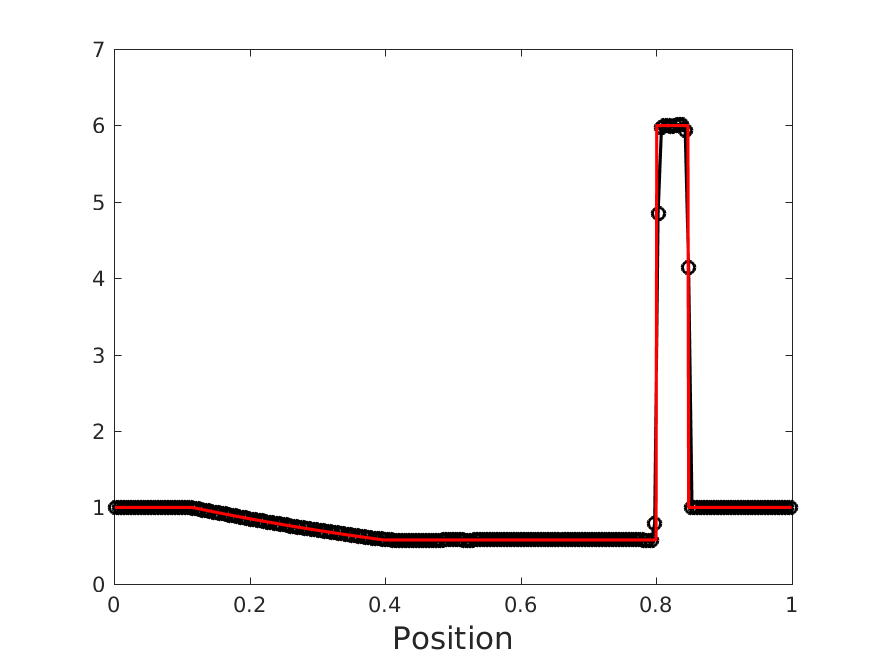
\includegraphics[width=.95\textwidth]{RiemannProblem_d5.png}
	\begin{tabular}{cc}
      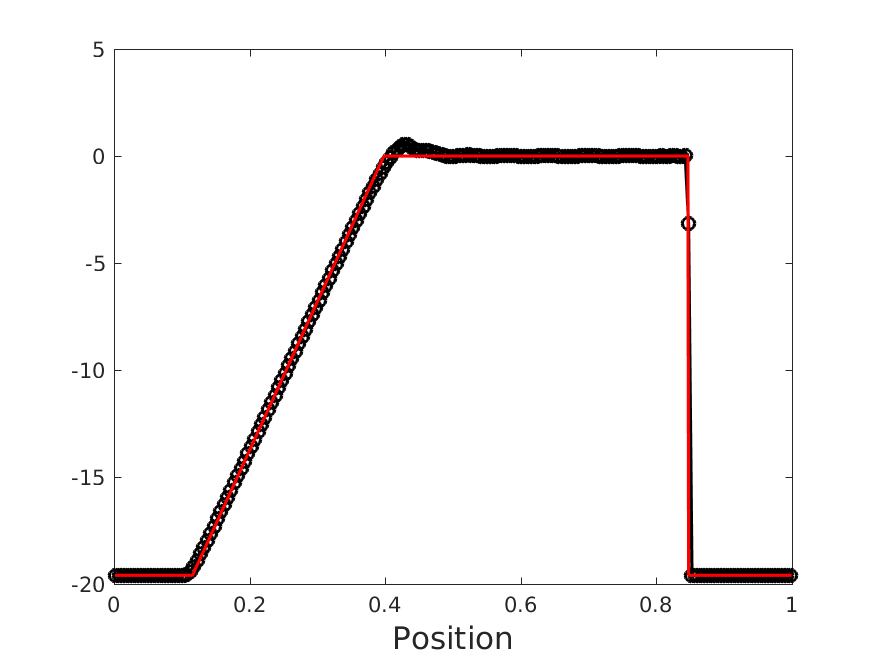
\includegraphics[width=.475\textwidth]{RiemannProblem_v5.png} &
	  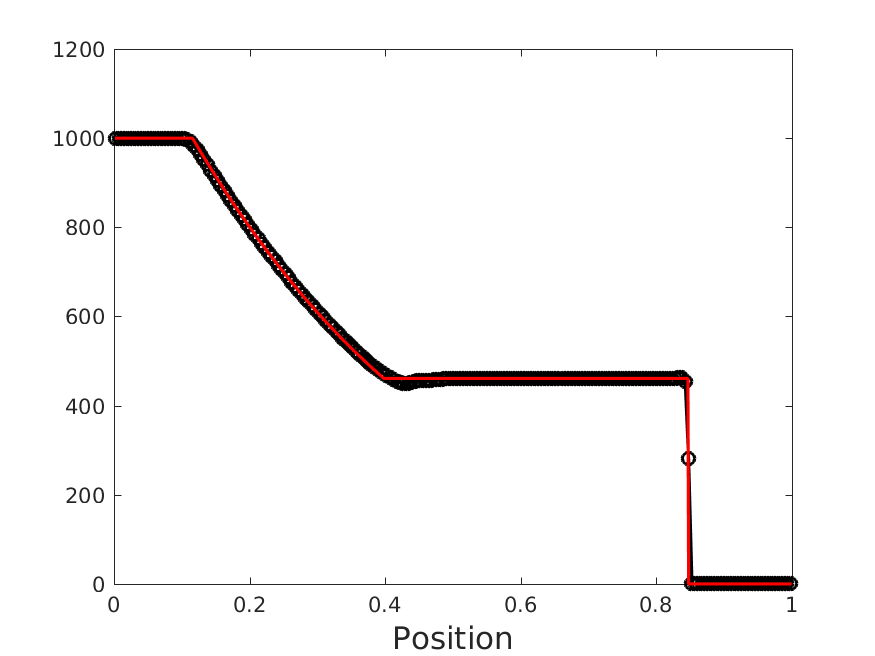
\includegraphics[width=.475\textwidth]{RiemannProblem_p5.png}
	\end{tabular}	
  \end{center}
  \caption{Results showing the density (top), velocity (bottom left), and pressure (bottom right) for the Riemann Problem at $t=0.012$, computed with 200 cells and the third order integration method (black), and the exact solution, obtained with Toro's Riemann solver (red).}
  \label{fig:Riemann}
\end{figure}

\subsubsection{Interacting Blast Waves}

\begin{figure}[h]
  \begin{center}
     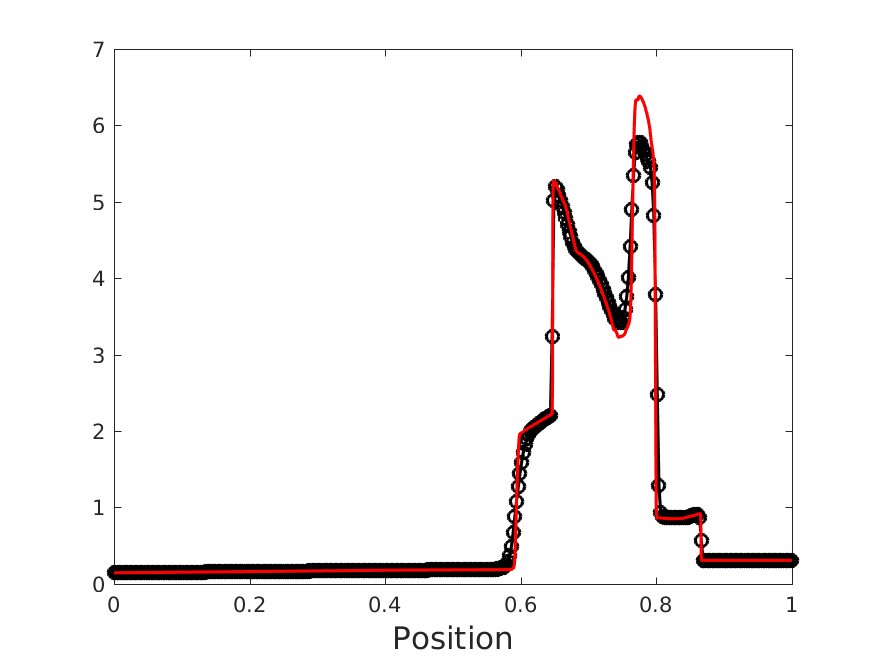
\includegraphics[width=.95\textwidth]{BlastD.png}	
	\begin{tabular}{cc}
     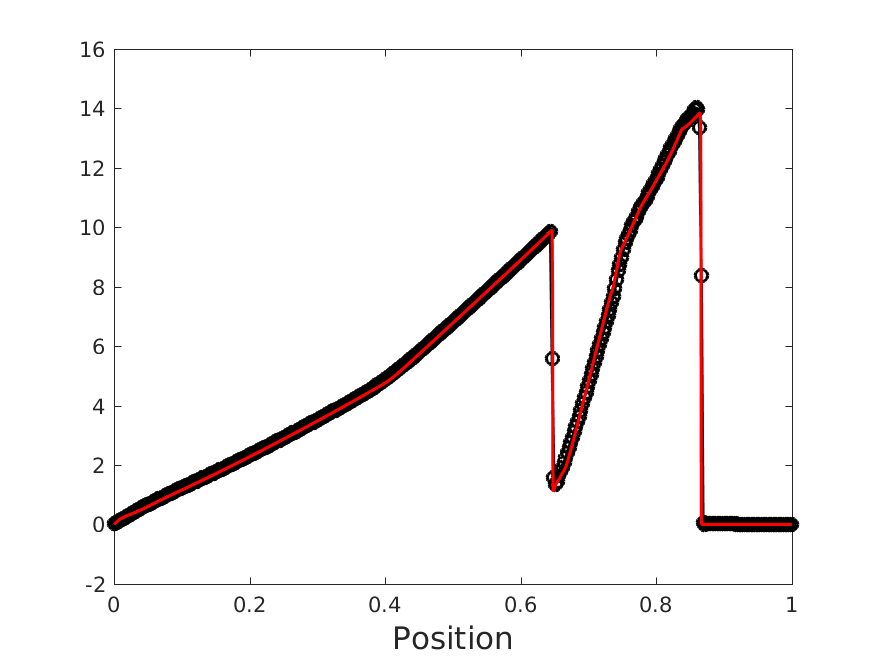
\includegraphics[width=.475\textwidth]{BlastV.png}
     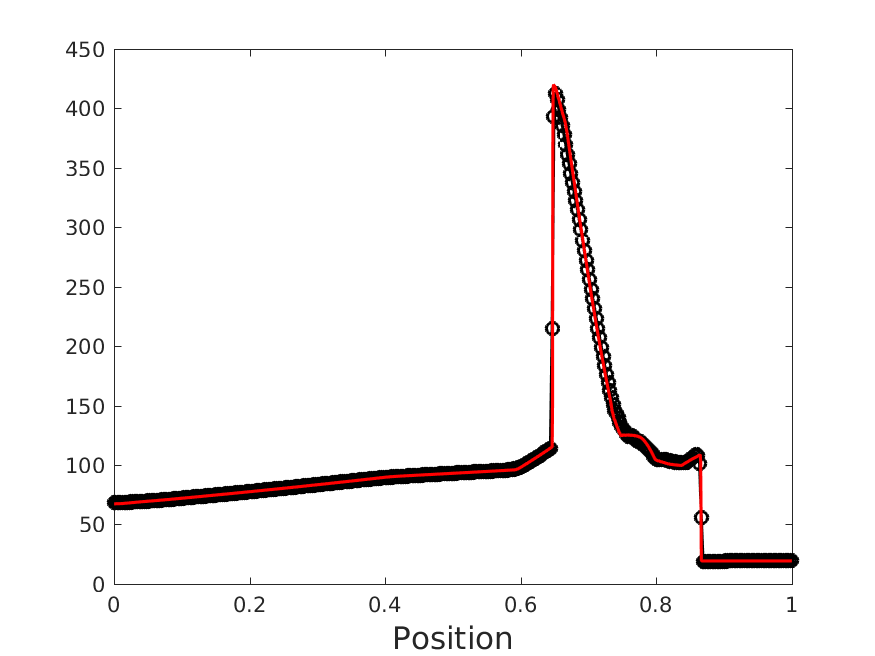
\includegraphics[width=.475\textwidth]{BlastP.png}	
    \end{tabular}
  \end{center}
  \caption{Results showing the density (top), velocity (bottom left), and pressure (bottom right) for the Woodward-Collela blast wave problem at $t=0.038$, computed with the 400 cells (black) and 2000 cells (red).}
  \label{fig:Blast}
\end{figure}
\clearpage
\subsubsection{Shock-Entropy Wave Interaction}

\begin{figure}[h]
  \begin{center}
	\begin{tabular}{cc}
      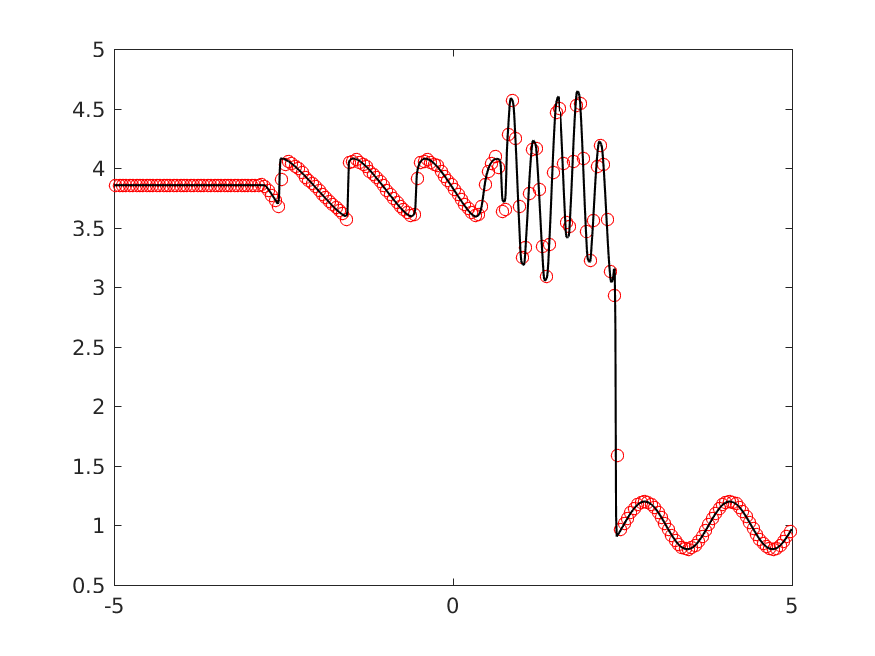
\includegraphics[width=.475\textwidth]{den.png} &
	  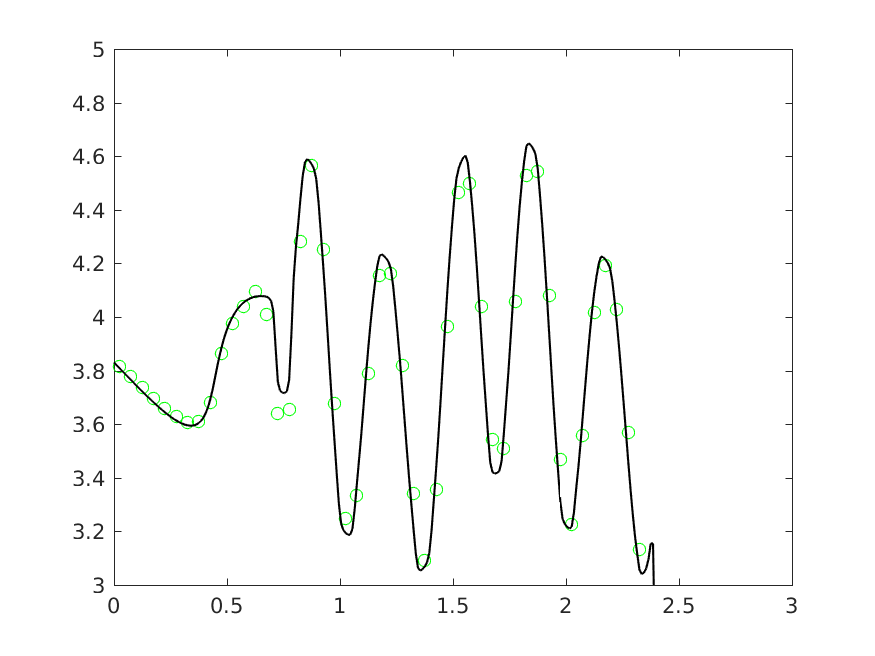
\includegraphics[width=.475\textwidth]{denzoom.png}
	\end{tabular}
  \end{center}
  \caption{Results showing the density for the Shock Entropy Wave problem at $t=1.8$, computed with 200 cells (green) and 1000 cells (black).}
  \label{fig:shock}
\end{figure}

\subsubsection{Sedov Blast Wave}

\subsubsection{Riemann Problem with Tabulated Nuclear EoS}

\subsection{Gravity Problems}

\subsubsection{Homogeneous Sphere}

\subsubsection{Hydrostatic Polytrope}

\subsubsection{Homologous Collapse}

\subsubsection{Evrard's Collapse Test}

\subsubsection{Stationary Accretion Shock}

\section{Miniapp: Adiabatic Collapse of Stellar Iron Core}
\label{sec:MiniApp}

\section{Summary and Conclusions}

\bibliographystyle{apj}
\bibliography{../References/references.bib}

\appendix

\section{Euler Equations in Commonly Used Coordinate Systems}
\label{app:CurvilinearEuler}

\subsection{Cylindrical Coordinates}

Mass conservation equation
\begin{equation}
  \pderiv{\rho}{t}
  +\f{1}{R}\pderiv{}{R}\Big(R\,\rho\,v^{1}\Big)
  +\pderiv{}{z}\Big(\rho\,v^{2}\Big)
  +\pderiv{}{\phi}\Big(\rho\,v^{3}\Big)=0,
\end{equation}
momentum conservation equation ($R$-component)
\begin{equation}
  \pderiv{\big(\rho\,v_{1}\big)}{t}
  +\f{1}{R}\pderiv{}{R}\Big(R\,\big(\rho\,v_{1}\,v^{1}+p\big)\Big)
  +\pderiv{}{z}\Big(\rho\,v_{1}\,v^{2}\Big)
  +\pderiv{}{\phi}\Big(\rho\,v_{1}\,v^{3}\Big)
  =\f{\big(\rho\,v_{3}\,v^{3}+p\big)}{R}-\rho\pderiv{\Phi}{R},
\end{equation}
momentum conservation equation ($z$-component)
\begin{equation}
  \pderiv{\big(\rho\,v_{2}\big)}{t}
  +\f{1}{R}\pderiv{}{R}\Big(R\,\rho\,v_{2}\,v^{1}\Big)
  +\pderiv{}{z}\Big(\rho\,v_{2}\,v^{2}+p\Big)
  +\pderiv{}{\phi}\Big(\rho\,v_{2}\,v^{3}\Big)=-\rho\pderiv{\Phi}{z},
\end{equation}
momentum conservation equation ($\phi$-component)
\begin{equation}
  \pderiv{\big(\rho\,v_{3}\big)}{t}
  +\f{1}{R}\pderiv{}{R}\Big(R\,\rho\,v_{3}\,v^{1}\Big)
  +\pderiv{}{z}\Big(\rho\,v_{3}\,v^{2}\Big)
  +\pderiv{}{\phi}\Big(\rho\,v_{3}\,v^{3}+p\Big)
  =-\rho\pderiv{\Phi}{\phi},
\end{equation}
energy equation
\begin{equation}
  \pderiv{E}{t}+\f{1}{R}\pderiv{}{R}\Big(\,R\,\big(E+p\big)\,v^{1}\,\Big)+\pderiv{}{z}\Big(\,\big(E+p\big)\,v^{2}\,\Big)+\pderiv{}{\phi}\Big(\,\big(E+p\big)\,v^{3}\,\Big)=-\rho\,v^{i}\pderiv{\Phi}{x^{i}},
\end{equation}
electron conservation equation
\begin{equation}
  \pderiv{n_{e}}{t}
  +\f{1}{R}\pderiv{}{R}\Big(R\,n_{e}\,v^{1}\Big)
  +\pderiv{}{z}\Big(n_{e}\,v^{2}\Big)
  +\pderiv{}{\phi}\Big(n_{e}\,v^{3}\Big)=0.  
\end{equation}

\subsection{Spherical Coordinates}

Mass conservation equation
\begin{equation}
  \pderiv{\rho}{t}
  +\f{1}{r^{2}}\pderiv{}{r}\Big(r^{2}\,\rho\,v^{1}\Big)
  +\f{1}{\sin\theta}\pderiv{}{\theta}\Big(\sin\theta\,\rho\,v^{2}\Big)
  +\pderiv{}{\phi}\Big(\rho\,v^{3}\Big)=0,
\end{equation}
momentum conservation equation ($r$-component)
\begin{equation}
  \pderiv{\big(\rho\,v_{1}\big)}{t}
  +\f{1}{r^{2}}\pderiv{}{r}\Big(r^{2}\,\big(\rho\,v_{1}\,v^{1}+p\big)\Big)
  +\f{1}{\sin\theta}\pderiv{}{\theta}\Big(\sin\theta\,\rho\,v_{1}\,v^{2}\Big)
  +\pderiv{}{\phi}\Big(\rho\,v_{1}\,v^{3}\Big)
  =\f{\rho(v_{2}v^{2}+v_{3}v^{3})+2p}{r}-\rho\pderiv{\Phi}{r},
\end{equation}
momentum conservation equation ($\theta$-component)
\begin{equation}
  \pderiv{\big(\rho\,v_{2}\big)}{t}
  +\f{1}{r^{2}}\pderiv{}{r}\Big(r^{2}\,\rho\,v_{2}\,v^{1}\Big)
  +\f{1}{\sin\theta}\pderiv{}{\theta}\Big(\sin\theta\,\big(\rho\,v_{2}\,v^{2}+p\big)\Big)
  +\pderiv{}{\phi}\Big(\rho\,v_{2}\,v^{3}\Big)
  =\big(\rho\,v_{3}v^{3}+p\big)\cot\theta-\rho\pderiv{\Phi}{\theta},
\end{equation}
momentum conservation equation ($\phi$-component)
\begin{equation}
  \pderiv{\big(\rho\,v_{3}\big)}{t}
  +\f{1}{r^{2}}\pderiv{}{r}\Big(\,r^{2}\,\rho\,v_{3}\,v^{1}\,\Big)
  +\f{1}{\sin\theta}\pderiv{}{\theta}\Big(\sin\theta\,\rho\,v_{3}\,v^{2}\Big)
  +\pderiv{}{\phi}\Big(\rho\,v_{3}\,v^{3}+p\Big)
  =-\rho\pderiv{\Phi}{\phi},
\end{equation}
energy equation
\begin{equation}
  \pderiv{E}{t}
  +\f{1}{r^{2}}\pderiv{}{r}\Big(r^{2}\,\big(E+p\big)\,v^{1}\Big)
  +\f{1}{\sin\theta}\pderiv{}{\theta}\Big(\sin\theta\,\big(E+p\big)\,v^{2}\Big)
  +\pderiv{}{\phi}\Big(\big(E+p\big)\,v^{3}\Big)=-\rho\,v^{i}\pderiv{\Phi}{x^{i}},
\end{equation}
electron conservation equation
\begin{equation}
  \pderiv{n_{e}}{t}
  +\f{1}{r^{2}}\pderiv{}{r}\Big(r^{2}\,n_{e}\,v^{1}\Big)
  +\f{1}{\sin\theta}\pderiv{}{\theta}\Big(\sin\theta\,n_{e}\,v^{2}\Big)
  +\pderiv{}{\phi}\Big(n_{e}\,v^{3}\Big)=0.  
\end{equation}

\section{Characteristic Decomposition}
\label{app:Characteristic}

Here we list eigenvalues and eigenvectors of the extended Euler equations in Eq.~\eqref{eq:extendedEulerCompact}.  
Let the vector of conserved variables be $\bU=(\rho,m_{1},m_{2},m_{3},E,n)^{T}$ and the flux vectors
\begin{align}
  \bF^{1}(\bU)
  &=\big(\,m_{1},\,m_{1}^{2}/\rho+p,\,m_{1}m_{2}/\rho,\,m_{1}\,m_{3}/\rho,\,(E+p)\,m_{1}/\rho,\,n\,m_{1}/\rho\,\big)^{T}, \\
  \bF^{2}(\bU)
  &=, \\
  \bF^{3}(\bU)
  &=.
\end{align}
The vector of primitive variables is $\bP=(\rho,v_{1},v_{2},v_{3},e,n)^{T}$.  
We have $v_{i}=m_{i}/\rho$ ($i=1,2,3$) and $e=E-\f{m^{2}}{2\,\rho}$, where $m^{2}=m_{1}^{2}+m_{2}^{2}+m_{3}^{2}$.  
The pressure is a function of the primitive variables $\rho$, $e$, and $n$; $p=p(\rho,e,n)$

The flux Jacobian matrices are given by
\begin{align}
  \pderiv{\bF^{1}(\bU)}{\bU}
  =
  \left(
  \begin{array}{cccccc}
  0 & 1 & 0 & 0 & 0 & 0 \\
  \big(\,p_{\rho}+\f{1}{2}p_{e}v^{2}\,\big)-v_{1}^{2} & \big(\,2-p_{e}\,\big)\,v_{1} & -p_{e}\,v_{2} & -p_{e}\,v_{3} & p_{e} & p_{n} \\
  - v_{1}v_{2} & v_{2} & v_{3} & 0 & 0 & 0 \\
  - v_{1}v_{3} & v_{3} & 0 & v_{1} & 0 & 0 \\
  \big[\big(p_{\rho}+\f{1}{2}p_{e}v^{2}\big)-H\big]\,v_{1} & H-p_{e}v_{1}^{2} & -p_{e}v_{1}v_{2} & -p_{e}v_{1}v_{3} & (1+p_{e})\,v_{1} & p_{n}\,v_{1} \\
  -n\,v_{1}/\rho & n/\rho & 0 & 0 & 0 & v_{1}
  \end{array}
  \right),
\end{align}
where $v^{2}=v_{1}^{2}+v_{2}^{2}+v_{3}^{2}$, $H=(E+p)/\rho$, $p_{\rho}=(\partial p/\partial \rho)$, $p_{e}=(\partial p/\partial e)$, and $p_{n}=(\partial p/\partial n)$.  
(For the ideal gas law, $p=p(e)=(\gamma-1)\,e$, we have $p_{\rho}=(\gamma-1)\f{1}{2}v^{2}$, $p_{e}=(\gamma-1)$, and $p_{n}=0$.)

\end{document}
